\lab{Nearest Neighbor Search}{Nearest Neighbor Search}
\label{lab:NNS}

\objective{Teach about branch and bound and the curse of dimensionality using the nearest neighbor search problem.}

\section*{The Nearest Neighbor Search Problem}

You move into a city that has several post offices.
You want to know which one is the closest.
This problem is  known as the nearest neighbor search problem or the post-office problem.
The general problem is to find the closest of a set of points to any new point.

This has many applications which include computer vision, pattern recognition, internet marketing and data compression.

The naive way to solve this problem is to check the distance of all the data against the point.

\begin{problem}
Write a function that solves the nearest neighbor search problem by exhaustively checking all the distances.
The function should take in the set of points that is the data and a single point.
The output should be the distance to the closest data point and the index of that point.
Your function should be able to take in data in an arbitrary dimension.
\end{problem}

The complexity of this algorithm is $O(kn)$.
Where  is the $k$ number of dimensions and $n$ is the number of data points.

\section*{K-D Trees}

A faster way to solve this problem is to build a k-d tree and search the k-d tree for the nearest neighbor. 

A k-d tree is a binary tree where the nodes to the left of parent node have a lower value in the i-th dimension and the nodes to the right of the parent node have a greater value in the i-th dimension.
Which dimension you split the nodes alternates at different levels.
In the $3$ dimensional case the root node is divided in the $x$ dimension, children in the $y$ dimension, grandchildren in the $z$ dimension, and the great-grandchildren in the $x$ dimension and so on.
Each node stores its location, left child and right child.
This requires sorting at each level so the complexity is $O(n log^2(n))$, but we only need to build the k-d tree once and after that we can query it as many times as we want.

Included is a function that takes in a set of data and builds k-d tree.
The leaf nodes' children are  python's ``None" object.

The search of the tree is done recursively.
Our search function will accept a parent node on which to search, a search point to which we want to find the nearest neighbor, the current best point, the current best distance, and a dimension $i$.
The search function should return the best point and best distance currently held in the algorithm.
We start the algorithm on the root node of the tree using it's point and distance to the search point as the best point and best distance, and start with $0$ as the first dimension.


For each recursive step, we first check if the euclidean distance between the parent node's point to the search point is less than the current best.
If so, we update it the best distance and best point to match the parent node.


We then compare the values in the $i$-th dimension of the search point and the parent's point.
If the search point's value is less than that of the parent node's point we recursively call the search function again on the left child of the parent node on the dimension $i+1$, flipping the dimension to $0$ if necessary, and set best point and best distance to it's output.
Then we have to check if the hypersphere around the point with radius being the current best distance crosses the dividing hyperplane created by the parent.
In code we accomplish this by adding the best distance to the point's value in the $i$-th dimension.
If this sum is greater than the parent's point value in the i-th dimension, we then search additionally the right child of the parent (using the dimension $i+1$) and update the best point and best distance to the output.


If the point's value was less than the parent's in th i-th dimension, we apply the last two steps mirrored to the right and left children.
We first search the right child with the $i+1$-th dimension and set the best point and best distance to the output.
We then check if the search point's value in the $i$-th dimension minus the best distance is less than the parent node's value in the $i$-th dimension. 
If it is, we will also search the left child one the $i+1$-th dimension and set the best point and best distance to the output.

Below the algorithm summarized in pseudo code 

\begin{algorithm}
\begin{algorithmic}[1]
\Procedure{KDSearch}{search\_point,parent\_node,b\_point,b\_distance,i}
    \If { Distance(search\_point,parent\_node.point) $<$ b\_distance }
        \State b\_point = parent\_node.point
        \State b\_distance = Distance from search\_point to parent\_node.point
    \EndIf

    \If{search\_point[i] $<$ parent\_node.point[i]}
        \State b\_point, b\_distance =
            \State KDSearch(search\_point,parent\_node.left\_child,b\_point,b\_distance,i+1)
        \If { search\_point[i] + b\_distance $geq$ parent\_node.point} 
            \State b\_point, b\_distance = 
                \State KDSearch(search\_point,parent\_node.right\_child,b\_point,b\_distance,i+1)
        \EndIf
    \Else
        \State b\_point, b\_distance = 
            \State KDSearch(search\_point,parent\_node.right\_child,b\_point,b\_distance,i+1)
        \If {search\_point[i] + b\_distance $leq$ parent\_node.point} 
            \State b\_point, b\_distance = 
                \State KDSearch(search\_point,parent\_node.left\_child,b\_point,b\_distance,i+1)
        \EndIf
    \EndIf
\EndProcedure
\end{algorithmic}
\caption{Nearest Neighbor}
\label{alg:nearestneighbor}
\end{algorithm}


\begin{problem}
Write a function that solves the nearest neighbor search problem by searching through a k-d tree.
The function should take in k-d tree and a single point.
The output should be the distance to the closest data point and the coordinates of that point. 
\end{problem}

\begin{problem}
Time both the functions you have created with the number of data points being $10,000-100,000$ every multiple of $10,000$ with $4$ dimensions.
Time only the searching of the k-d tree not the building of it.
Plot both times on the same plot.
How do the two algorithms compare?


\begin{figure}[H]
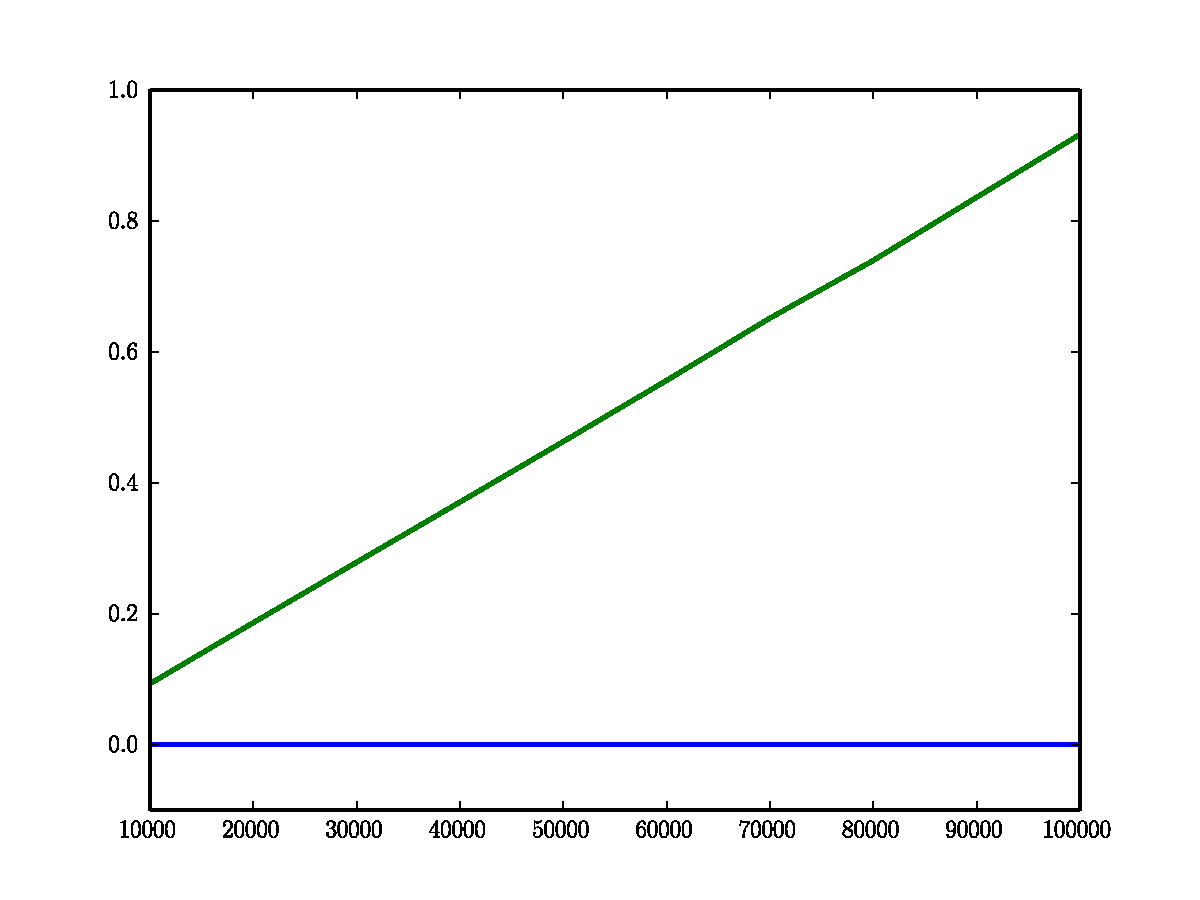
\includegraphics[width=\textwidth]{fourDTime.pdf}
\caption{Your graph should look like this.
The green line is the naive version and blue line is using a kd-tree.
As you can see the kd-tree is much faster.}
\label{fig:fourDTime}
\end{figure}
\end{problem}

The complexity of this algorithm is $O(klog(n))$ in optimal time.
Its worst case is $O(k*n^{1-\frac{1}{k}})$ where $k$ is the number of dimensions and $n$ is the number of points in the tree.
The reasons for this are discussed in the next section.

\section*{Curse of Dimensionality}

As you increase the number of dimensions the number of times that you have to go down both branches increases.
You get to the point where you eliminate very few points by using a k-d tree.

\begin{problem}
Time both algorithms for the number of data points being $10,000-100,000$ every multiple of $10,000$ with $20$ dimensions.
Plot both times on the same plot. Now how do the two algorithms compare?
\end{problem}

\begin{figure}[H]
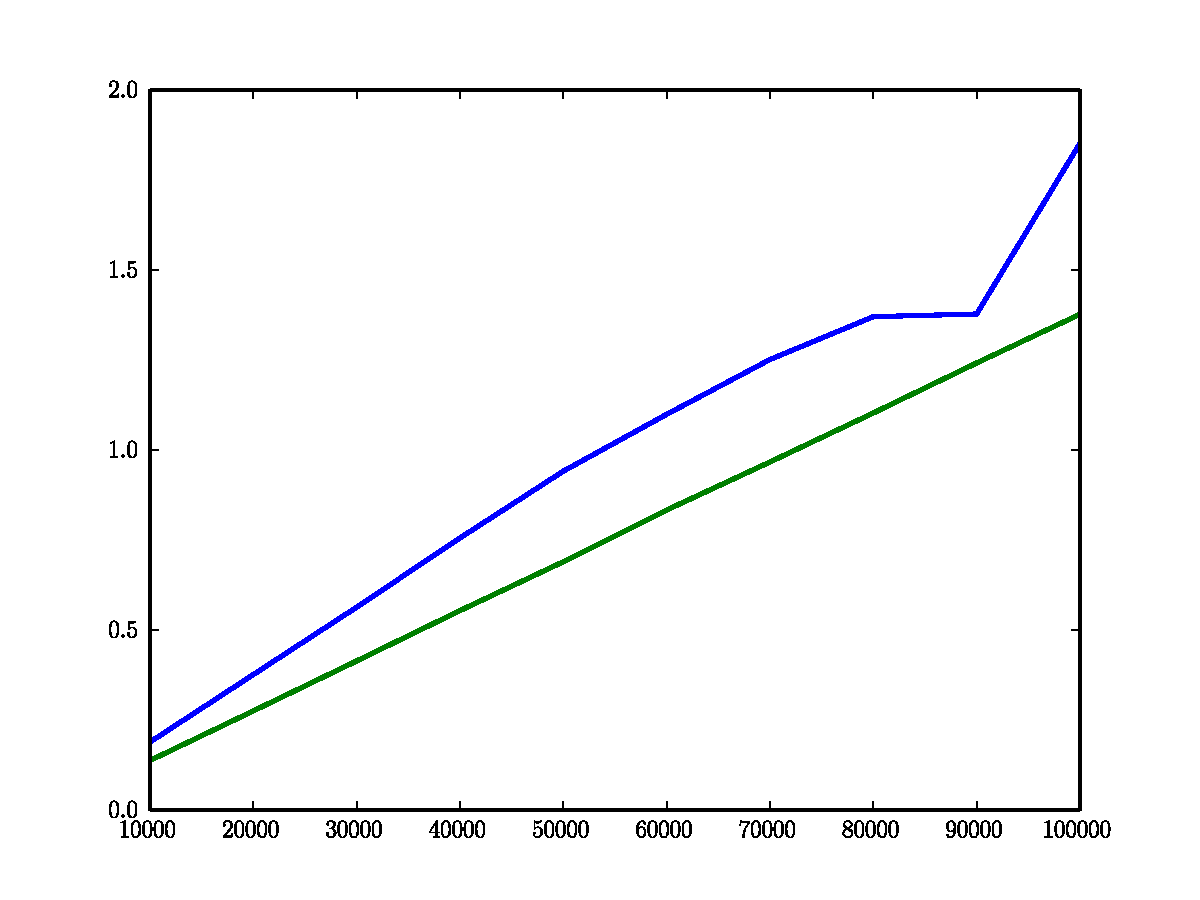
\includegraphics[width=\textwidth]{twentyDTime.pdf}
\caption{
Your graph should look like this.
The green line is the naive version and blue line is using a kd-tree.
As you can see the kd-tree is slightly slower than the naive version.}
\label{fig:twentyDTime}
\end{figure}

\begin{problem}
Time the SciPy built in function for searching a k-d tree (do not time the building of the kd-tree) for the number of dimensions points being $2-50$ with $20,000$ data points.
Plot the time.
What do you notice?
\li{from scipy.spatial import KDTree} will import the built in k-d tree.
Create the tree by \li{tree = KDTree(data)} and search it by \li{tree.query(point)}.

\li{scipy.spatial} includes a \li{cKDTree} object which is implemented in C.
Is it any better?

\begin{figure}[H]
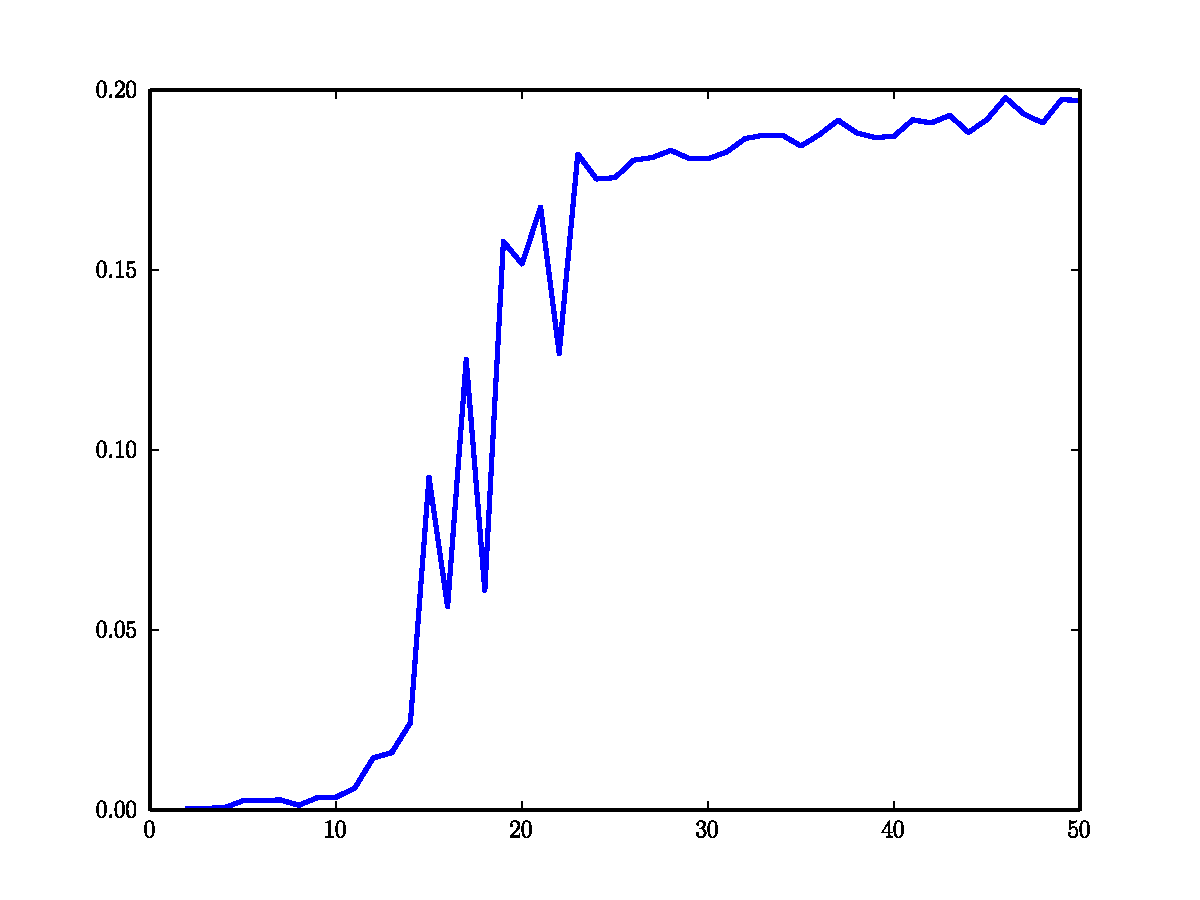
\includegraphics[width=\textwidth]{curseD.pdf}
\caption{
Your graph should look similar to this.
Around 15 dimensions the time jumps.
At that point using a kd-tree is not more effective than checking all the combinations.}
\end{figure}
\end{problem}

\section*{Classification}
A common problem is correctly classifying data.  
Suppose that you have a ten marbles, five of which are blue with a green stripe and the other five red with a purple stripe.  
If your friend gave you an eleventh marble that was blue with a brown stripe, which group would you put it in?  
Probably you would include it with the other blue marbles.  
What if the marble that your friend gave you was blue with a purple stripe?  
This marble shares characteristics with both groups.  
Where you end up grouping it will depend on which characteristics are most important to you.

This is the intuitive classfication problem.  
If we have data that is already grouped into distinct sets, into which set do we put new data?  
Classification has myriad and sundry applications.  
In this lab we will use it in the context of optical character recognition.

\section*{Nearest Neighbor Classification}
We will now more formally describe the classification problem and explain the nearest neighbor classification algorithm.  
Suppose we have a collection of vectors $\{x_1, ..., x_m\}$ in $\R^n$ with corresponding labels $\{l_1, ..., l_k\}$ describing to which group each datum belongs.  
This collection of vectors and labels is called our training set.  
Each entry of a vector is called a feature and $n$ is the size of our feature set.  
For example, consider the following vectors in $\R^3$

\begin{center}
\begin{tabular}{cc}
$(2,0,0)$ & $1$ \\
$(3,0,0)$ & $1$ \\
$(0,3,0)$ & $2$ \\
$(0,2,0)$ & $2$ \\
$(1/10,2,0)$ & $2$ \\
$(0,0,4)$ & $3$ \\
$(0,0,7)$ & $3$ \\
\end{tabular}
\end{center}

If we also have a metric on our space, we may determine the distance between all of these points.  
If we are given a new datum and we wish to decide which of the three groups to include it in, one option is to choose the group to which its closest neighbor belongs.  
Let us use the euclidean metric to classify $(0,0,5)$ against our training set.  
We see that the distance from $(0,0,5)$ and $(0,0,4)$ is only $1$, while the distance to the remaining points is at least $2$.  
The label of $(0,0,4)$ is $3$, and so we assign $(0,0,5)$ the same label.

Now, what if we wished to classify $(5/2,5/2,0)$?  
This presents a problem since this point is equidistant from the points in label $1$ and label $2$.  
In such a case it is up to the programmer to decide how to break the tie.

One case we need to consider is when the data that we are using in our search are on different scales. 
For example, suppose we wished to classify people applying for a loan at a bank as `risky' or `safe.'  
Further suppose that we know their age, education level, current debt, and how many credit cards they have.  
We could encode their education level as integers between $0$ and $4$.

Suppose that Bob is 30 years old, well educated, has a debt of \$5000, and 3 credit cards.  
Let's say that James is 18 years old, barely out of high school, \$5000 dollars in debt, and owns 4 credit cards.  
If we were to use the Euclidean metric $d$ to measure how close Bob is to James, we would get a distance of
\[
d((30,4,5000,3),(18,0,5000,4)) = 12^2 + 4^2 + 1^2 = 161.
\]

However, if Alice is 29 years old, well educated, has a debt of \$4900, and 3 credit cards, then her distance from Bob is
\[
d((30,4,5000,3),(29,4,4900,3)) = 1^2 + 100^2 = 100001.
\]

Is James closer to Bob than Alice?  Most Banks would say no.  
In order to classify these individuals better, we need to measure distance differently. 
There are two different ways to handle this. 
The first solution is to scale the data before inputting it into our algorithm. 
In our previous example we could divide age by 100, education by 4, debt by 1000, and credit cards by 10 and then preform a nearest neighbor search on Bob. 
Then the distance from Bob to James is 
\[
d\left( \left( \frac{30}{100},\frac{4}{4},\frac{5000}{1000},\frac{3}{10} \right),\left(\frac{18}{100},\frac{0}{4},\frac{5000}{1000},\frac{4}{10}\right)\right) = .12^2 + 1^2 + .1^2 = 1.0244.
\]
while the distace from Alice to Bob is
\[
d\left(\left(\frac{30}{100},\frac{4}{4},\frac{5000}{1000},\frac{3}{10}\right),\left(\frac{29}{100},\frac{4}{4},\frac{4900}{1000},\frac{3}{10}\right)\right) = .1^2 + .01^2 = 0.0101.
\]
So now Bob is closer to Alice.

\begin{problem}
Write a function that takes in data points and the a vector that is used to be the scale. 
The function outputs the scaled data points. 
So if we were using it for our baking example it would take in the array representing the data Alice, Bob and James (where each person is a row) and the vector $[100,4,1000,10]$ and output the scaled data of Alice, Bob and James.
\end{problem}

Another alternative is to change the metric we use to measure distance with. 
In both the examples above we used the Euclidean metric to measure distance. 
Suppose we wished to apply the Euclidean metric to data set of colors.
We could map each color to an integer, say red to 1, violet to 2, blue to 3, green to 4, yellow to 5, and orange to 6. 
If we use Euclidean metric green is closer to red than orange is when we'd probably consider orange to be the same distance from red as violet is. 
In this case the Euclidean metric is not satisfactory and so we might create a new metric to measure the distance between colors. 

\section*{K-Nearest Neighbor Classification}
Often we can improve the accuracy of a classifier by looking for other points besides the nearest neighbor.  
Instead, we may choose an arbitrary number $k$ and give the point to be classified the majority label in from it's $k$ nearest neighbors. 

There are pitfalls to this approach.  
Consider a point that's closest neighbor has the label $0$.  
If we only considered the nearest neighbor, then we would be finished.  
However, what if the next $10$ nearest neighbors all had the label $1$?  
Do you think that we should still classify the point as $0$?  
What if the nearest point has a distance of $0.1$ and the next $10$ points have a distance of at least $100$?  
The answer to these questions depend on the kind of data we are working with and the metric that we choose.  
One should ensure to consider how to treat situations like this when working on classification algorithms.


The sklearn library has a neighbors module with a class KNeighborsClassifier for solving the $k$ nearest neighbors problem
\begin{lstlisting}
from sklearn import neighbors
nbrs = neighbors.KNeighborsClassifier(n_neighbors=8, weights='distance', p=2)
\end{lstlisting}

The \li{neighbors.KNeighborsClassifier} sets up the knearestnieghbor algorithm. 
\li{n_neighbors} is how many neighbors you would like to find and \li{weights} specifies how you would like to weight the neighbors you have to make the classification. 
Weights can be \li{'uniform'}, where the majority classification of the $k$ nearest neighbors determines the new data point's classification, or \li{'distance'}, where the neighbors nearer to the point have more weight than those farther away. 
The argument \li{p} correpsods to the distance metric. 
For this lab we will use \li{p=2} which is the Euclidean distance.  

\begin{lstlisting}
nbrs.fit(points, labels)
\end{lstlisting}
Points and labels are your training data. 
The \li{fit} function makes \li{nrbs} create a data structure containing those points and labels ready to be queried. 

\begin{lstlisting}
nbrs.predict(testpoints)
\end{lstlisting}

The function \li{predict} takes in points to classify and outputs their respective labels.  
%More information about this package can be found at http://scikit-learn.org/stable/modules/neighbors.html.
\begin{problem}
Get the post office handwritten digit data set. Load them with
\begin{lstlisting}
labels, points, testlabels, testpoints = np.load('PostalData.npz').items()
\end{lstlisting}
This contains a training set and a test set. 
When you load the data the first entry of each array will be a name. 
So \li{points[1]} and \li{labels[1]} point to the actual points and labels you want to use. 
Each point is a  image that is $28 \times 28$ matrix of pixels that has been flattened. 
The corresponding label indicates which number was written.  
Try classifying the testpoints with \li{n_neighbors} as 4 and then as 10 and with \li{weights} \li{'uniform'} and then \li{'distance'}. Then do the classfication with \li{n_neighbors} being 1. 
For each one return a report indicating how your classifier performs in terms of misclassifications as a percentange (testlabels are the true labels that correspond to the testpoints). 
Which combination gives the most correct classifications?
(You may wish to streamline this process by writting a function that takes in \li{n_neighbors} and \li{weights} as arguments calls the neighbors functions appropriately)


A similar classification process is used by the United States Postal Service to automatically determine the zip code to send a letter to.

\begin{figure}[H]
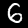
\includegraphics[width=.25\textwidth]{Example.png}
\caption{An example of the number 6 taken from the data set}
\end{figure}
\end{problem}


